\documentclass{article}
\usepackage{graphicx}
\usepackage{float}
\usepackage{hyperref}
%\usepackage[latin1]{inputenc} 
%\usepackage[T1]{fontenc}
%\usepackage{english}
\title{Batch and Stream Processing: Realtime Analysis of Big Data}
\date{}
\author{Marcel Stolin \\ marcelpascal.stolin@studenti.unitn.it}

\def\Eq#1{\eqref{#1}}
\def\Sec#1{Section~\ref{#1}}
\def\Ex#1{Example~\ref{#1}}
\def\Chap#1{Chapter~\ref{#1}}
\def\Part#1{Part~\ref{#1}}
\def\Fig#1{Figure~\ref{#1}}
\def\Lst#1{Listing~\ref{#1}}
\def\Tab#1{Table~\ref{#1}}
\def\Alg#1{Algorithm~\ref{#1}}
\def\Page#1{Page~\pageref{#1}}

\begin{document}


\maketitle


\begin{abstract}
Since the beginning of Big Data, batch processing was the most popular choice for processing large amounts of generated data. These existing processing technologies are not suitable to process the large amount of data we face today. Research works developed a variety of technologies that focus on stream processing. Stream processing technologies bring significant performance improvements and new opportunities to handle Big Data. In this paper, we discuss the differences of batch and stream processing and we explore existing batch and stream processing technologies. We also explain the new possibilities that stream processing make possible.
\end{abstract}

\section{Part 1}\label{sec:01_part1}

\subsection{Introduction}\label{subsec:01_part1_intro}
% Intro to the HTTP server
In the second lecture of the course, an implementation of a basic HTTP server with the name \textit{TinyHttpd} was introduced.
The functionality of the HTTP server is limited to opening \texttt{.html} files and delivering the content via the HTTP 1.1 protocol to the client.


% Problem statement
The task of part 1 of the first assignment, is to extend the \textit{TinyHttpd} implementation by implementing the functionality to launch an external process. Therefore, the client sends a request via the URL \texttt{http://localhost:8000/process/reverse?par1=ROMA}. Then, the server executes an external Java process, which reverses the string \texttt{ROMA}, given in the query \texttt{?par1=ROMA}, and responses the result of the external Java process to the client via HTTP 1.1.


% Domain description
Given the above mentioned task description, the following steps have to be implemented:
\begin{enumerate}
\item Create a Java application, called \textit{StringReverser}, which takes a valid String as input and returns the reversed string
\item Extend the \textit{TinyHttpd} implementation to launch external processes when requested by client via the URL \texttt{http://localhost:8000/process/PROCESS\_NAME?PROCESS\_PARAMETERS}.
\end{enumerate}

\subsection{Conceptual Design}\label{subsec:01_part1_design}
Given the problem statement introduced in \Sec{subsec:01_part1_intro}, a new application called \textit{StringReverser} needs to be implemented, and the \textit{TinyHttpd} server has to be extended in a way to launch an external Java process.

\subsubsection{StringReverser}
% Design of the StringReverser
The \textit{StringReverser} application is a simple terminal application. It takes any valid String as an input and returns the reversed String as the output. It can be executed via the console, for example the command \texttt{\$ java -jar StringReverser.jar ROMA} should responses the string \textit{AMOR}.

\subsubsection{TinyHttpd}
% Extension of TinyHttpd
Whenever the client makes a request via the URL \texttt{http://localhost:8000/process/PROCESS\_NAME?PROCESS\_PARAMETERS}, the server is supposed to start an external Java process, waits for the output of the process, and responses the process output to the user.
% URL
The client has the possibilities to specify which process has to be executed. Given the URL \texttt{http://localhost:8000/process/reverse?par1=ROMA}, the user explicitly requests to launch the \textit{reverse} process with the given query \texttt{par1=ROMA} as the process input.
% Input
It is important to mention, that each process takes individual parameters as input. For the above mentioned \texttt{StringReverser}, only the value of the first parameter in the given query is important. All other parameters, and the parameter key, are therefore ignored.

\subsection{Implementation}\label{subsec:01_part1_impl}
To implement given conceptual design, The Java programming language is used in version OpenJDK 17\footnote{JDK 17 - \url{https://openjdk.java.net/projects/jdk/17/} (Accessed: 02/10/2021)}.

\subsubsection{StringReverser}
% Implementation of StringReverser
The application \textit{StringReverser} is a simple Java project. It is composed of a single Java class called \texttt{StringReverser} as shown in \Fig{fig:01_part1_impl_stringreverser_structure}.
% Implementation of StringReverser
The source code is shown in \Fig{fig:01_part1_impl_stringreverser_implementation}, and it consists of a \texttt{main} method and a method called \texttt{reverseString}.
% The main method
The main method will be executed, when the application is launched via the terminal. Additionally, it checks if a String is been given as input, and if the input is valid. Otherwise, it will return an error message and exists with system code 0. If the input is a valid string, it will call the \texttt{reverseString} method, and returns the result as the output.
% The reverse method
The \texttt{reverseMethod} is responsible to reverse the given input. Therefore, it uses the \texttt{StringBuilder}\footnote{StringBuilder - \url{https://docs.oracle.com/javase/7/docs/api/java/lang/StringBuilder.html} (Accessed: 02/10/2021)} class to reverse the String.

% StringReverser project structure
\begin{figure}[h]
\centering
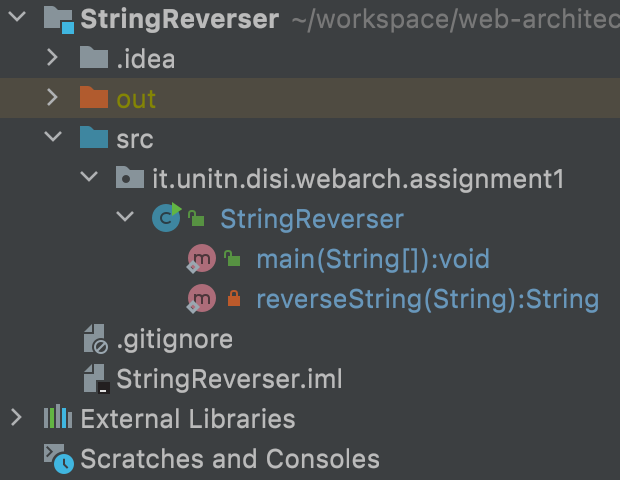
\includegraphics[scale=0.4]{images/StringReverserStrct}
\caption{Project structure of the \texttt{StringReverser} application}
\label{fig:01_part1_impl_stringreverser_structure}
\end{figure}

% StringReverser implementation
\begin{figure}[h]
\centering
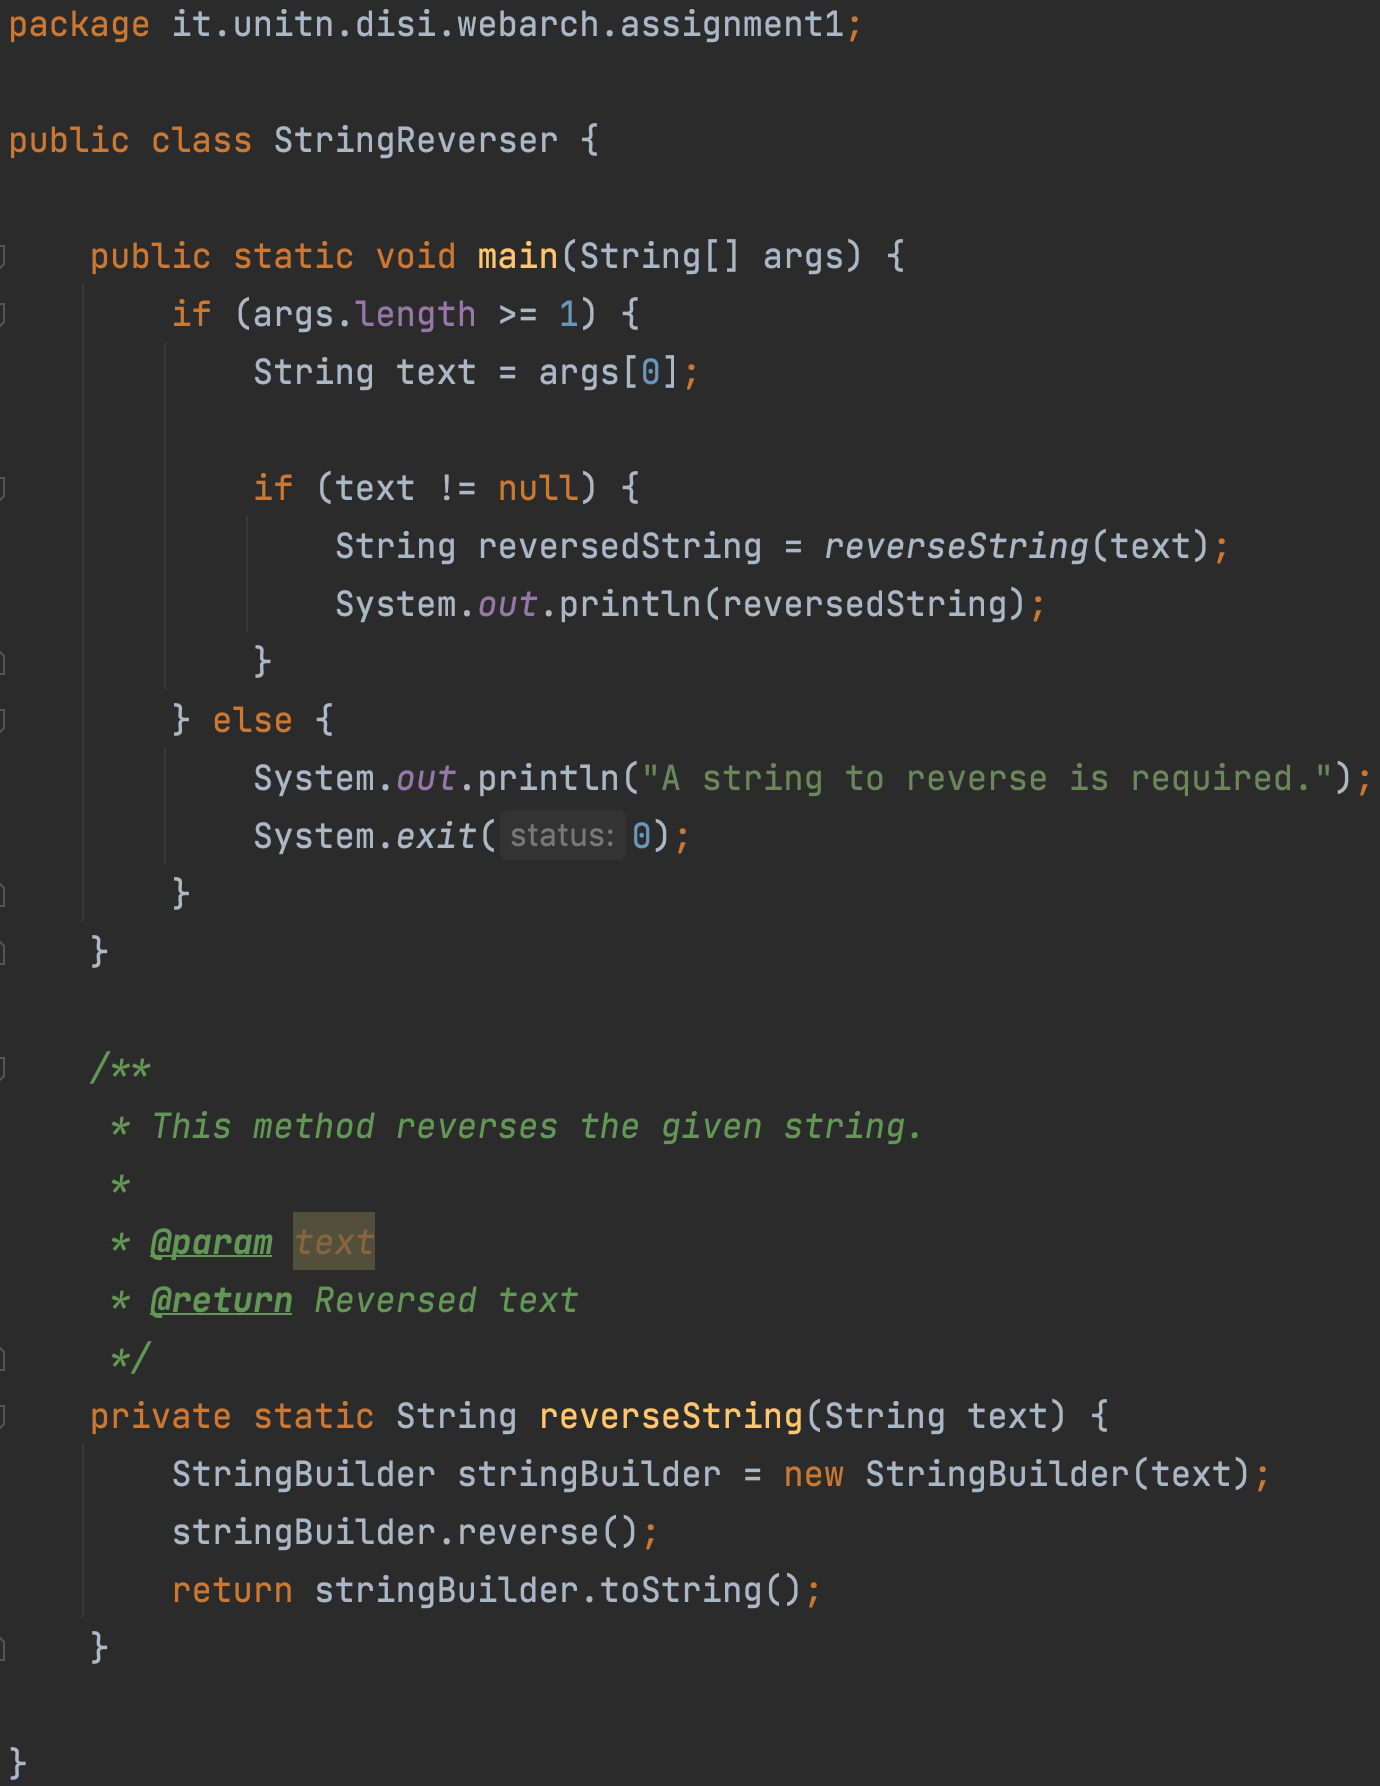
\includegraphics[scale=0.4]{images/StringReverserImpl}
\caption{Implementation of the \texttt{StringReverser} class}
\label{fig:01_part1_impl_stringreverser_implementation}
\end{figure}

% Execution
\Fig{fig:01_part1_impl_stringreverser_execution} shows the execution of the \textit{StringReverser} application. The \texttt{.jar} artifact was created using the IntelliJ IDEA\footnote{Create your first Java application - \url{https://www.jetbrains.com/help/idea/creating-and-running-your-first-java-application.html} (Accessed: 02/10/2021)}.
% Failure execution
If the input is invalid, the \texttt{StringReverser} will print an error message to the terminal and exit with system code 0, as shown in \Fig{fig:01_part1_impl_stringreverser_execution_fail}.

% StringReverser execution
\begin{figure}[h]
\centering
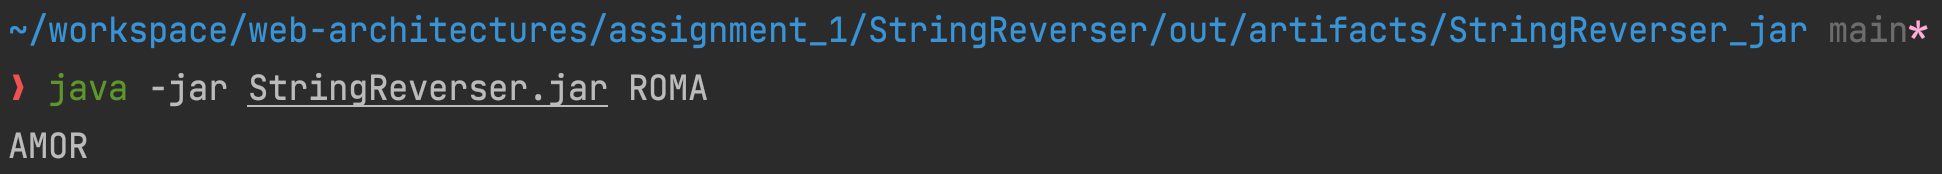
\includegraphics[scale=0.4]{images/StringReverserExec}
\caption{Successful execution of the \textit{StringReverser} application}
\label{fig:01_part1_impl_stringreverser_execution}
\end{figure}

% StringReverser execution fail
\begin{figure}[h]
\centering
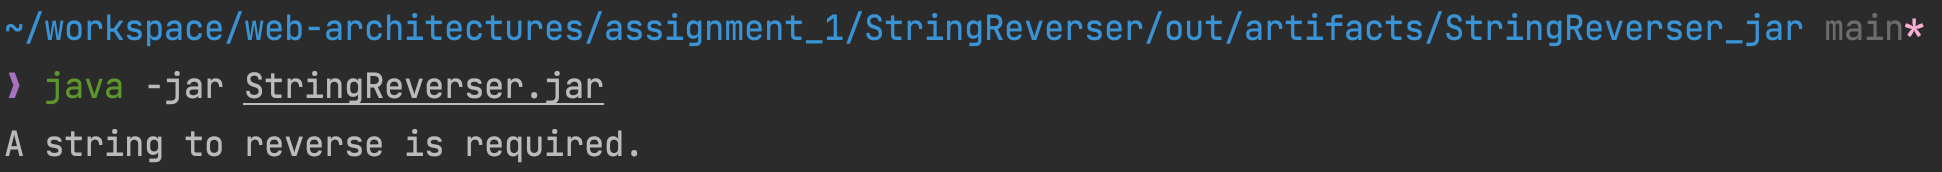
\includegraphics[scale=0.4]{images/StringReverserExecFail}
\caption{Execution of the \textit{StringReverser} application without an input}
\label{fig:01_part1_impl_stringreverser_execution_fail}
\end{figure}

\subsubsection{TinyHttpd}
% Extension of TinyHttpd
The foundation of the TinyHttpd project is provided by the Professor. It has to be extended to launch external Java processes, and deliver the process output to the client. As mentioned in SEC DESIGN, the client sends a HTTP request via the URL \texttt{http://localhost:8000/process/PROCESS\_NAME?PROCESS\_PARAMETERS}. Currently, the implementation responses with the content of the requested HTML file, if available. Otherwise, an 404 HTTP response is send to the client.


% Parse request
To be able to detect, if the client wants to launch an external Java process, the request has to be parsed accordingly. Therefore, the first step is to extend the existing code base with a \texttt{RequestParser} class. The \texttt{RequestParser} class is able to parse a HTTP request into its parts. Given the request \texttt{GET /process/reverse?param=roma HTTP/1.1}, it is composed of the HTTP method (\texttt{GET}), the path (\texttt{/process/reverse?param=roma}), and the HTTP protocol version (\texttt{HTTP/1.1}). Furthermore, the path has an additional query attached (?param=roma). FIG XY shows the implementation of the \texttt{RequestParser} class.
% Then start process
After the \texttt{RequestParser} has successfully parsed the clients request, it is possible to check, via an \texttt{if} statement, if the user requested the path \textit{/request/PROCESS\_NAME}. If yes, the server executes the requested process, and sends a response accordingly. Otherwise, if the client has not requested to perform a Java process, the server tries to open the HTML file according to the given path and responses the HTML content to the client. The implementation of this procedure is shown in \Fig{fig:01_part1_impl_tinyhttpd_parsing}.
% Parsign Implementation
\begin{figure}[h]
\centering
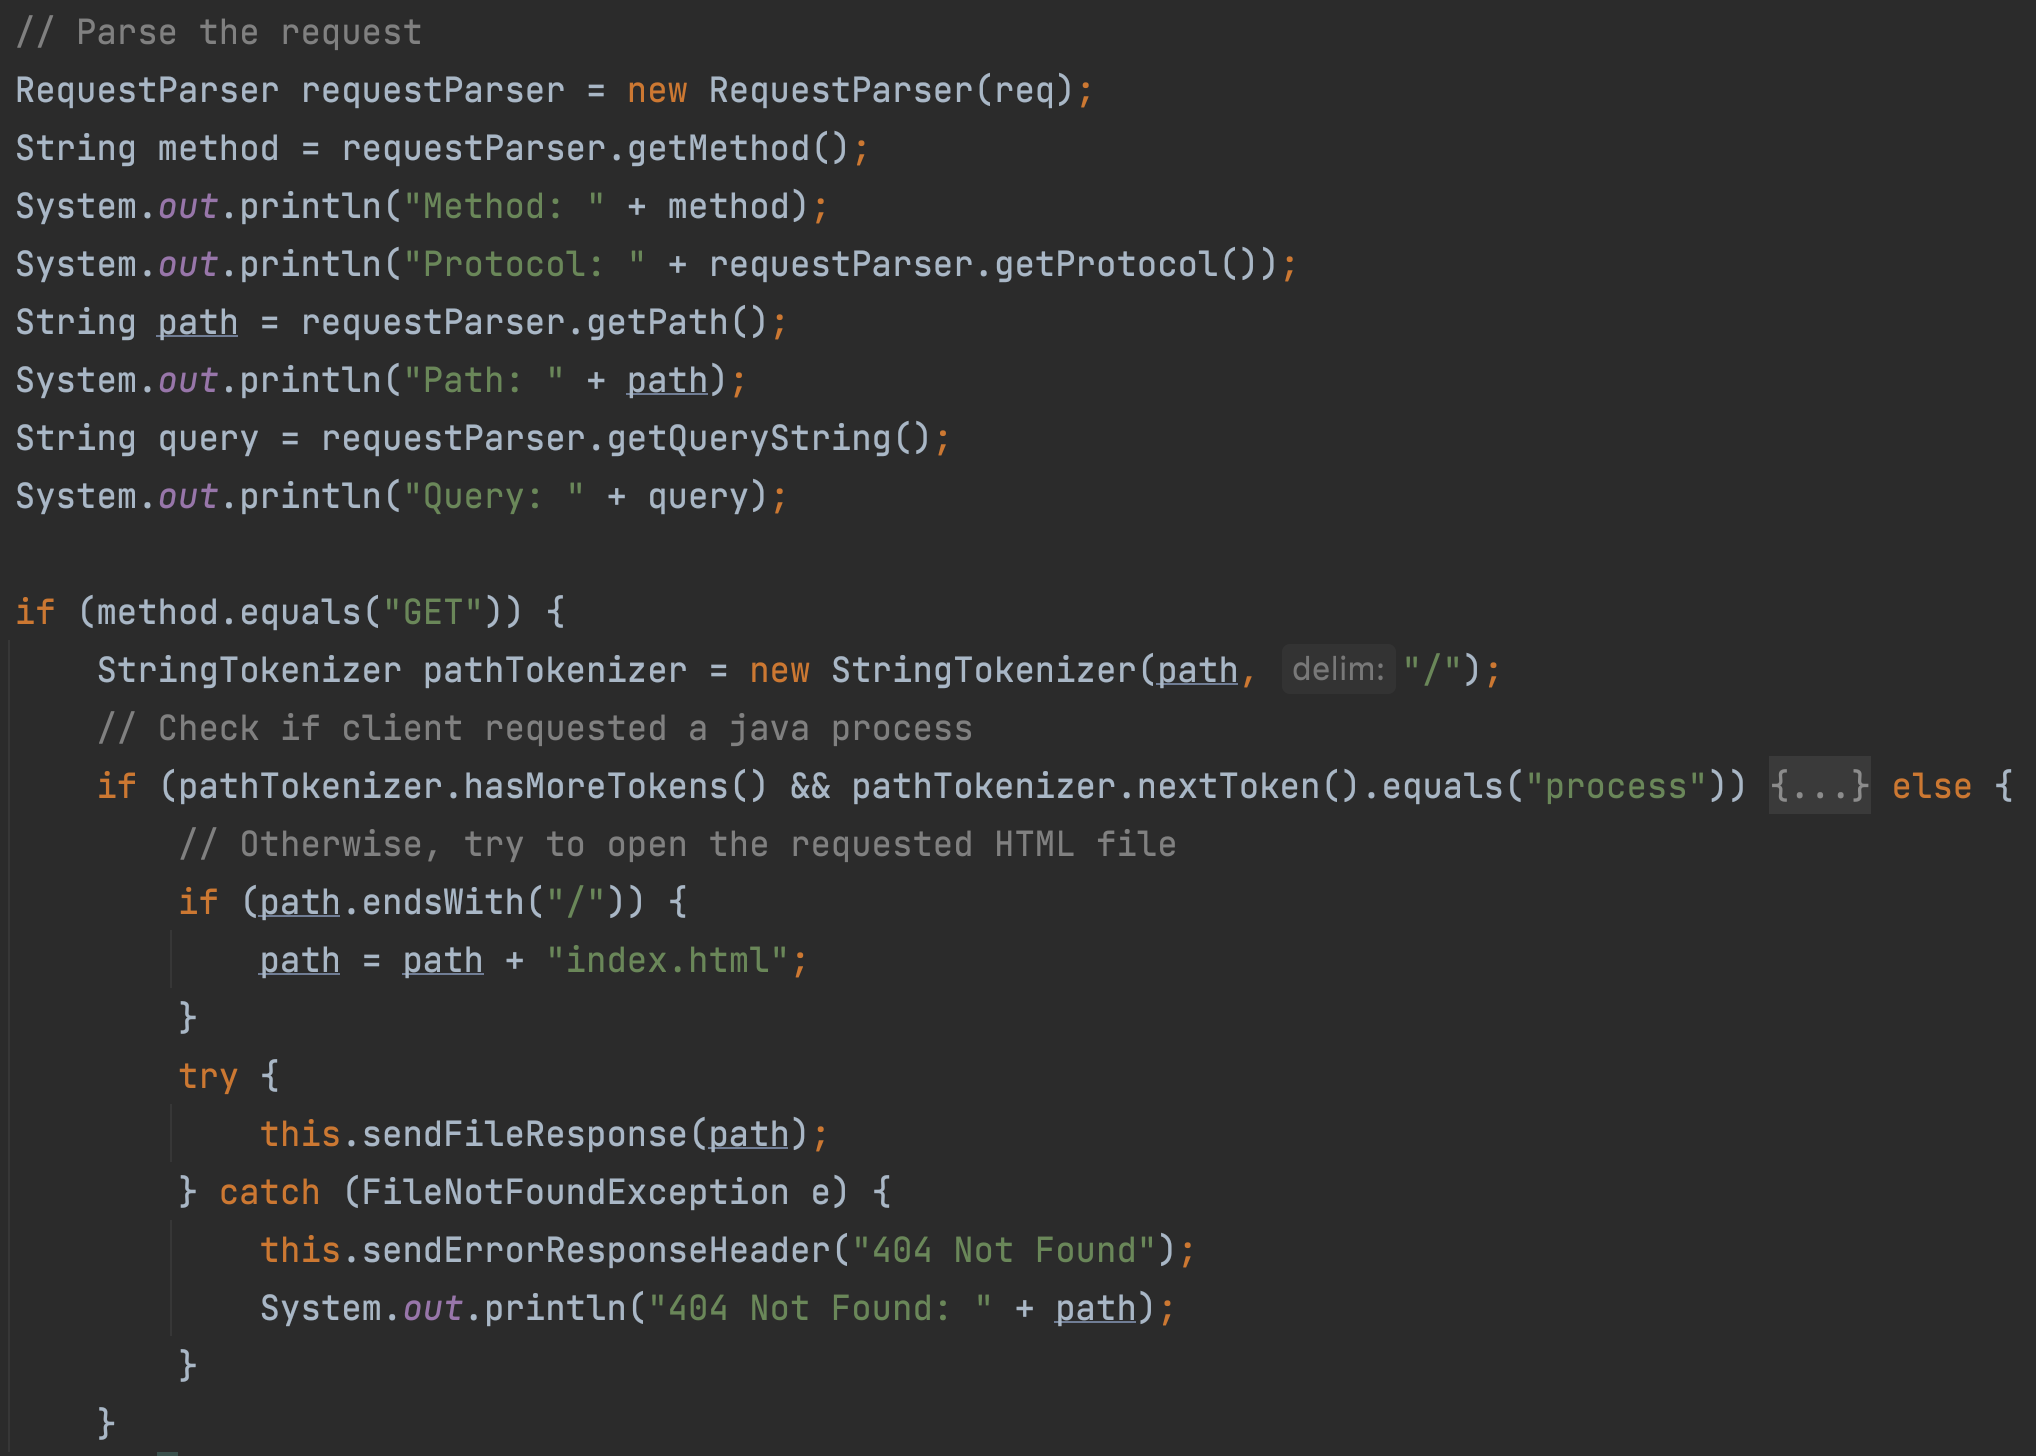
\includegraphics[scale=0.4]{images/TinyHttpdParsing}
\caption{Execution of the \textit{StringReverser} application without an input}
\label{fig:01_part1_impl_tinyhttpd_parsing}
\end{figure}

% Start the requestes process


\subsection{Conclusion}\label{subsec:01_part1_concl}


%===============
%===============


\section{Part 2}\label{sec:02_part2}

\subsection{Introduction}\label{subsec:02_part2_intro}

\subsection{Design}\label{subsec:02_part2_design}

\subsection{Implementation}\label{subsec:02_part2_impl}

\subsection{Conclusion}\label{subsec:02_part2_concl}

\bibliographystyle{plain}
\bibliography{mybib}

\end{document}